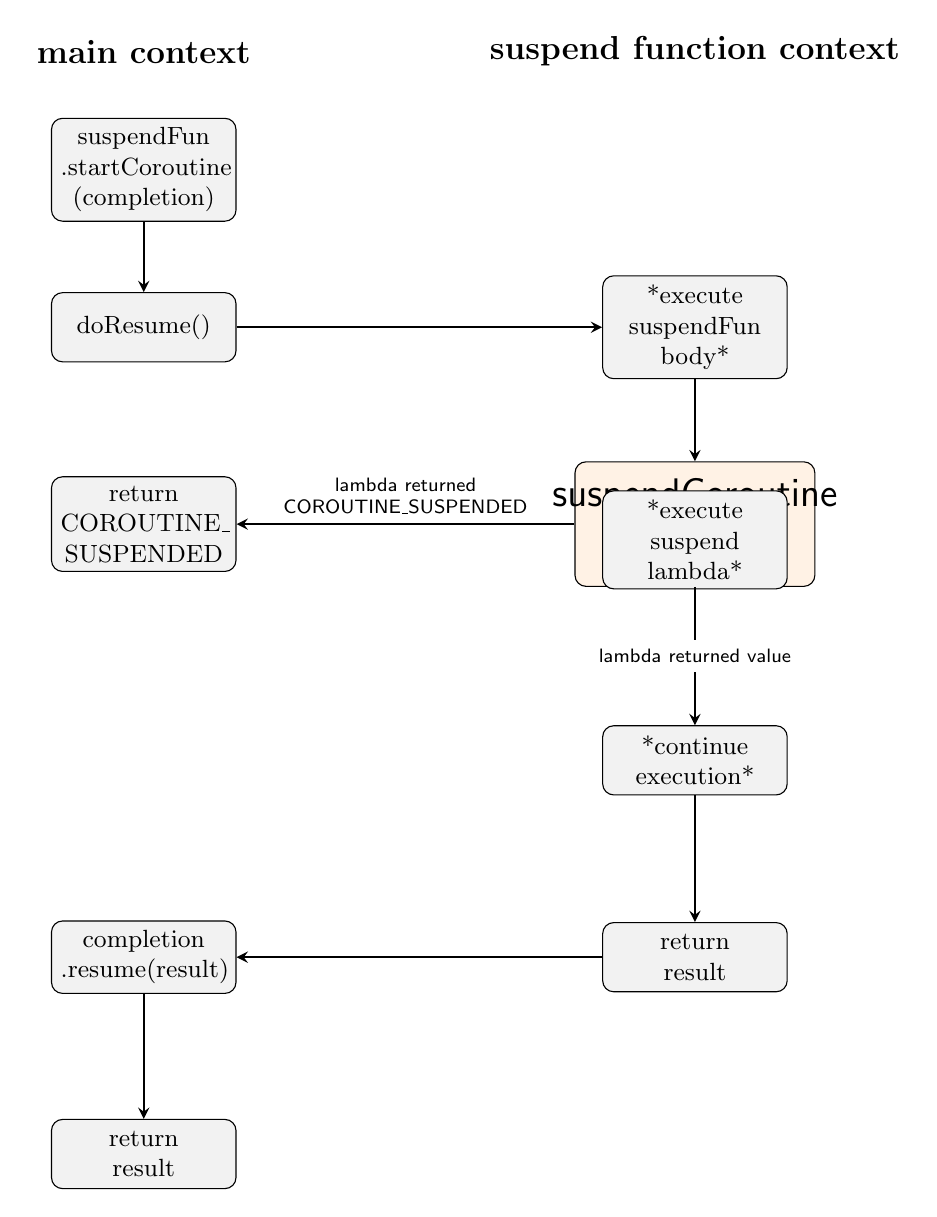
\begin{tikzpicture}[
    node distance=0.8cm and 3cm,
    every node/.style={font=\small},
    block/.style={rectangle, draw, fill=blue!10, text width=5em, text centered, rounded corners, minimum height=2.5em},
    decision/.style={diamond, draw, fill=yellow!10, text width=4em, text centered, aspect=2, inner sep=1pt},
    action/.style={rectangle, draw, fill=green!10, text width=6em, text centered, rounded corners, minimum height=2.5em},
    suspend/.style={rectangle, draw, fill=orange!20, text width=6em, text centered, rounded corners, minimum height=2.5em},
    title/.style={font=\large\bfseries},
    note/.style={rectangle, draw, fill=gray!10, text width=6em, text centered, rounded corners, minimum height=2.5em},
    container/.style={rectangle, draw, fill=orange!10, text width=8em, minimum height=4.5em, rounded corners},
    arrow/.style={->, >=stealth, thick},
    transfer/.style={->, >=stealth, thick, dashed},
    solidarrow/.style={->, >=stealth, thick},
    label/.style={font=\scriptsize}
]
% -------------------------
% Column Titles
% -------------------------
    \node[title] (title1) at (0, 0) {main context};
    \node[title] (title2) at (7, 0) {suspend function context};

% -------------------------
% Left Column Nodes
% -------------------------
    \node[note] (n1) at (0, -1.5) {suspendFun\\.startCoroutine\\(completion)};
    \node[note] (n2) at (0, -3.5) {doResume()};
    \node[note] (n3) at (0, -6) {return\\COROUTINE\_\\SUSPENDED};
    \node[note] (n4) at (0, -11.5) {completion\\.resume(result)};
    \node[note] (n5) at (0, -14) {return\\result};

% -------------------------
% Right Column Nodes
% -------------------------
    \node[note] (n6) at (7, -3.5) {*execute\\suspendFun\\body*};

% Container Box for suspendCoroutine
    \node[container] (n7_box) at (7, -6) {};
    \node[anchor=north, font=\sffamily\Large, inner sep=6pt] at (n7_box.north) {suspendCoroutine};
    \node[note] (n7_note) at (7, -6.2) {*execute\\suspend\\lambda*};

    \node[note] (n8) at (7, -9) {*continue\\execution*};
    \node[note] (n9) at (7, -11.5) {return\\result};

% -------------------------
% Arrows & Routing
% -------------------------
    \draw[arrow] (n1) -- (n2);
    \draw[arrow] (n2) -- (n6);
    \draw[arrow] (n6) -- (n7_box);

% Left arrow from container to return SUSPENDED
    \draw[arrow] (n7_box.west) -- node[above, align=center, font=\sffamily\scriptsize] {lambda returned \\ COROUTINE\_SUSPENDED} (n3.east);

% Down arrow from container to continue execution
    \draw[arrow] (n7_box.south) -- node[fill=white, align=center, font=\sffamily\scriptsize] {lambda returned value} (n8.north);

    \draw[arrow] (n8) -- (n9);
    \draw[arrow] (n9) -- (n4);
    \draw[arrow] (n4) -- (n5);
\end{tikzpicture}
